%!TEX root = ../notes.tex
\section{March 8, 2022}
\subsection{Legendre Symbol \emph{continued}}
\begin{example}\label{example:legendre-symbol}
    Determine if $219$ is a quadratic residue mod $383$ (we note that $383$ is a prime).
    \begin{align*}
        \lege{219}{383} & = \lege{3}{383}\cdot\lege{73}{383}    \\
        \intertext{We now flip the Legendre Symbols using quadratic reciprocity:}
                        & = -\lege{383}{3} \cdot \lege{383}{73} \\
                        & = -\lege{2}{3} \cdot \lege{18}{73}    \\
                        & = 1\cdot \lege{18}{73}                \\
                        & = \lege{2}{73}\cdot\lege{9}{73}       \\
                        & = \lege{2}{73} = \boxed{1}
    \end{align*}
\end{example}
\begin{remark*}
    We must factor the top argument before beginning to flip using quadratic reciprocity.
\end{remark*}

\subsection{Proof of Quadratic Reciprocity}

Recall \cref{thm:qr}:
\begin{theorem*}[Law of Quadratic Reciprocity]
    Let $p, q\in\ZZ_+$ be distinct odd positive primes. Then
    \begin{equation*}
        \lege{p}{q}\lege{q}{p} = (-1)^{\frac{p-1}{2}\frac{q-1}{2}}
    \end{equation*}
    In other words,
    \[\lege{p}{q} = \lege{q}{p}\]
    if and only if at least one of $p, q$ is congruent to $1$ mod $4$.
\end{theorem*}

\begin{proof}[Proof of Quadratic Reciprocity (\cref{thm:qr}), using Gauss's Lemma (\cref{lemma:gauss-lemma})]
    \textsc{wlog}, let
    \begin{align*}
        P & = \left\{1, 2, \dots, \frac{p-1}{2}\right\},\quad N=-P, \\
        Q & = \left\{1, 2, \dots, \frac{q-1}{2}\right\}
    \end{align*}
    We write $\tilde P, \tilde N$ for $P\pmod{p}$ and $N\pmod{p}$ respectively, so that Gauss's lemma gives
    \[\lege{q}{p} = (-1)^\mu, \quad\text{where }\mu = |q\tilde P\cap\tilde N|\]
    In other words, $\mu$ is exactly the number of $x\in P$ such that $qx\equiv n\pmod{p}$ for some $n\in N$, and hence the number of $x\in P$ such that for $y\in \ZZ$, \[-\frac{p}{2} < qx - py < 0.\]
    We now specify more precisely which $y$ can possibly satisfy this condition. Solving these inequalities for $y$ gives
    \begin{align*}
        \frac{qx}{p} < y < \frac{qx}{p}+\frac{1}{2}.
    \end{align*}
    \otoh, since $x\leq \frac{p-1}{2}$ $\forall x\in P$, this gives
    \begin{align*}
        y < \frac{qx}{p}+\frac{1}{2} & \leq \frac{q(p-1)}{2p}+\frac{1}{2} \\
                                     & < \frac{q+1}{2}.
    \end{align*}
    Thus $0 < y < \frac{q+1}{2}$, which means that
    \[y\in Q = \left\{1, 2, \dots, \frac{q-1}{2}\right\}.\]
    We've shown that $\mu$ is the number of points $(x, y)\in P\times Q$ such that
    \[\frac{p}{2} < qx - py < 0.\]

    Switching $p$ and $q$, we also have
    \[\lege{p}{q} = (-1)^\eta\]
    where $\eta$ is the number of pairs
    \[(y, x)\in Q\times P\]
    such that
    \[-\frac{q}{2} < py - qx < 0\]
    which is exactly the number of pairs
    \[(x, y)\in P\times Q\]
    satisfying
    \[0 < qx - py < \frac{q}{2}\]
    (reflecting the inequality over $0$).

    We note that
    \[\lege{p}{q}\lege{q}{p} = (-1)^\mu (-1)^\eta = (-1)^{\mu+\eta}\]
    so all that remains is counting $\mu$ and $\eta$. And we have that $\mu + \eta$ is the number of ordered pairs $(x, y)\in P\times Q$ such that either
    \[-\frac{p}{2} < qx - py < 0 \text{ or } 0 < qx - py < \frac{q}{2}\]
    Noting that $qx - py\neq 0$ since $x$ and $y$ are from $P$ and $Q$ respectively, hence we can reduce this to
    \[-\frac{p}{2} < qx - py < \frac{q}{2}.\]
    Graphically, we are looking at:
    \begin{center}
        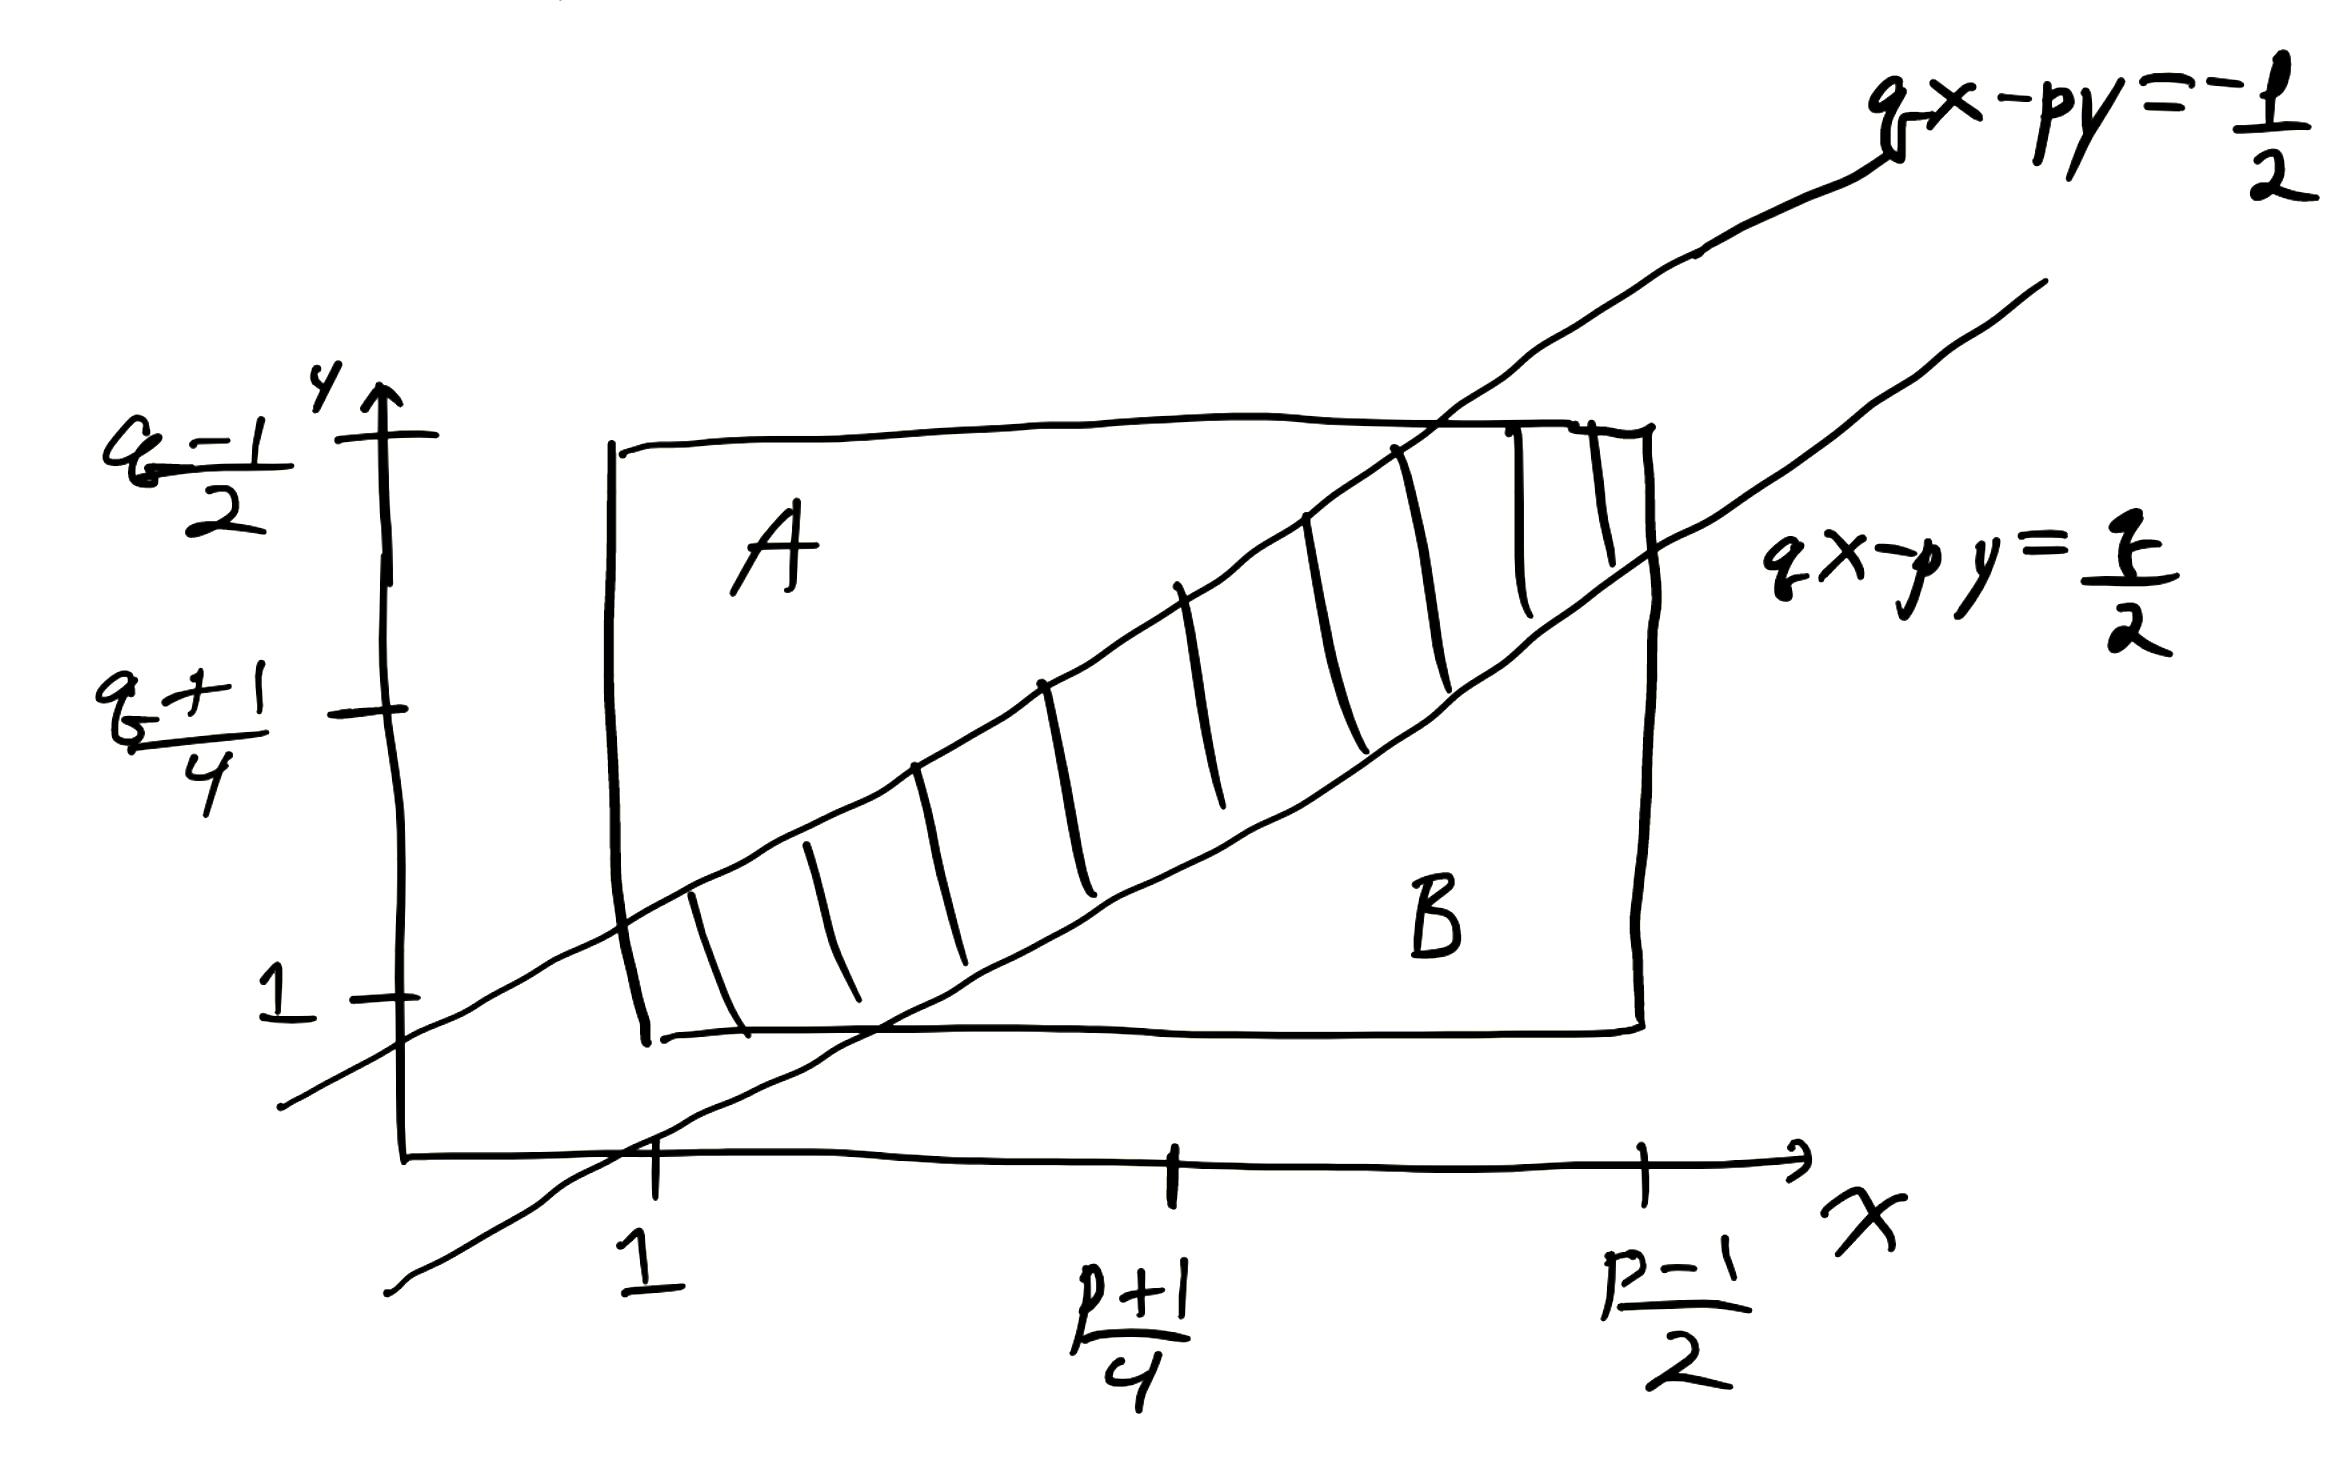
\includegraphics[width=0.8\textwidth]{images/qr-diagram.png}
    \end{center}

    where $\mu + \eta$ is the number of lattice points in the shaded region.

    If $\alpha$ is the number of lattice points in $A$ and $\beta$ the number of lattice points in $B$. Then
    \[\mu + \eta = \frac{p-1}{2}\frac{q-1}{2} - (\alpha + \beta)\]
    We show that $\alpha = \beta$ so that $\alpha + \beta \equiv 0\pmod{2}$.

    Let $\rho$ be the rotation given by rotating the rectangle about its center leaves it invariant.
    \[\rho(x, y) = \left(\frac{p+1}{2}-x, \frac{q+1}{2} - y\right)\]
    Quick check that
    \[qx - py < \frac{-p}{2} \Leftrightarrow qx' - py' > \frac{q}{2}\]

    Since $\rho$ maps lattice points to lattice points, then $\alpha = \beta$ which concludes the proof with a little extra handiwork.
\end{proof}

\subsection{Jacobi Symbol}
The Jacobi symbol generalizes the Legendre symbol.
\begin{definition}[Jacobi Symbol]
    Let $b$ be an odd positive integer and let $a\in\ZZ$. Write
    $b = p_1p_2\cdots p_m$, where $p_i$ are (not necessarily distinct) primes. Then we write
    \[\lege{a}{b} = \lege{a}{p_1}\lege{a}{p_2}\cdots \lege{a}{p_m}\]
    is called the \ul{Jacobi symbol}.
\end{definition}
We note some basic properties that the Jacobi symbol is totally multiplicative (on top and bottom!):
\begin{align*}
    \lege{a_1a_2}{b} & = \lege{a_1}{b}\lege{a_2}{b} \\
    \lege{a}{b_1b_2} & = \lege{a}{b_1}\lege{a}{b_2}
\end{align*}
\begin{remark*}
    Note that they're multiplicative \emph{fixing} either top or bottom. That is, they don't multiply like fractions.
\end{remark*}

\textbf{Warning!} $\lege{a}{b} = 1$ does not imply that $a$ is a quadratic residue modulo $b$ (since we could have $-1$'s from the factorization cancel out).

However, $\lege{a}{b} = -1$ \emph{does} imply that $a$ is a non-residue modulo $b$. (it is a non-residue mod at least one of prime factors of $b$).

\begin{example}
    \[\lege{2}{15} = \lege{2}{3}\lege{2}{5} = (-1)(-1) = 1\]
    but $2$ is not a quadratic residue modulo $15$.
\end{example}
\begin{proposition}[5.2.2 of Text]\label{prop:5.2.2}
    We have the following properties about the Jacobi symbol:
    \begin{enumerate}[(a)]
        \item \[\lege{-1}{b} = (-1)^{\frac{b-1}{2}}\]
        \item \[\lege{2}{b} = (-1)^{\frac{b^2 - 1}{8}}\]
        \item If $a, b\in\ZZ_+$, then
              \[\lege{a}{b}\lege{b}{a} = (-1)^{\frac{a-1}{2}\frac{b-1}{2}}\]
    \end{enumerate}
\end{proposition}